\lhead{附录: 试题}
\invisiblesection{摄动理论2012年期末试题}
\problemlist{\bf 摄动理论2012年期末试题\footnote{{\bf 说明:} 本试题是本人考试后立刻回忆出来的, 供后届同学参考.}}

\begin{enumerate}
\item 确定下列函数的阶, 并按大小排列($\varepsilon\rightarrow 0$)
\[
\ln\sinh\frac{1}{\varepsilon},\quad
\ln\csc\varepsilon,\quad
\exp\Big(\frac{\sqrt{1-\cos^2\varepsilon}}{-\sin\varepsilon^2}\Big),\:
\frac{1-\cos\varepsilon}{\varepsilon^{4/3}},\quad
\tan\sqrt{\varepsilon},\quad
\ln(2+\sin\varepsilon),\quad
\]
\[
\varepsilon\sin\varepsilon,\quad
\ln\bigg[1+\frac{\ln(1+1\varepsilon)}{1-\varepsilon}\bigg],\quad
\varepsilon^{1/2}(1-\cos\varepsilon)^{-1/2},\quad
\ln(1+\varepsilon)
\]

\vspace{0.5em}
\item 试求下述问题的首项解
\[
u''+\varepsilon u'+u +\varepsilon u^3 = 0
\]

\vspace{0.5em}
\item 试求下述问题的可解性条件.
\[
u'' + 4u= f(x),\:
u(0) = a, \:
u'(\pi/4)=b
\]

\vspace{0.5em}
\item 试求一致有效展开的首项
\[
\varepsilon y'' + xy' + xy = 0,\:
u(0)=\alpha,\:
y(1) = \beta
\]
\end{enumerate} 

\newpage
\invisiblesection{渐进分析2011年期末试题}
\problemlist{\bf 渐进分析2011年期末试题\footnote{{\bf 说明:} 2012年的试题与2011年试题相仿.}} 
\begin{center}
\fbox{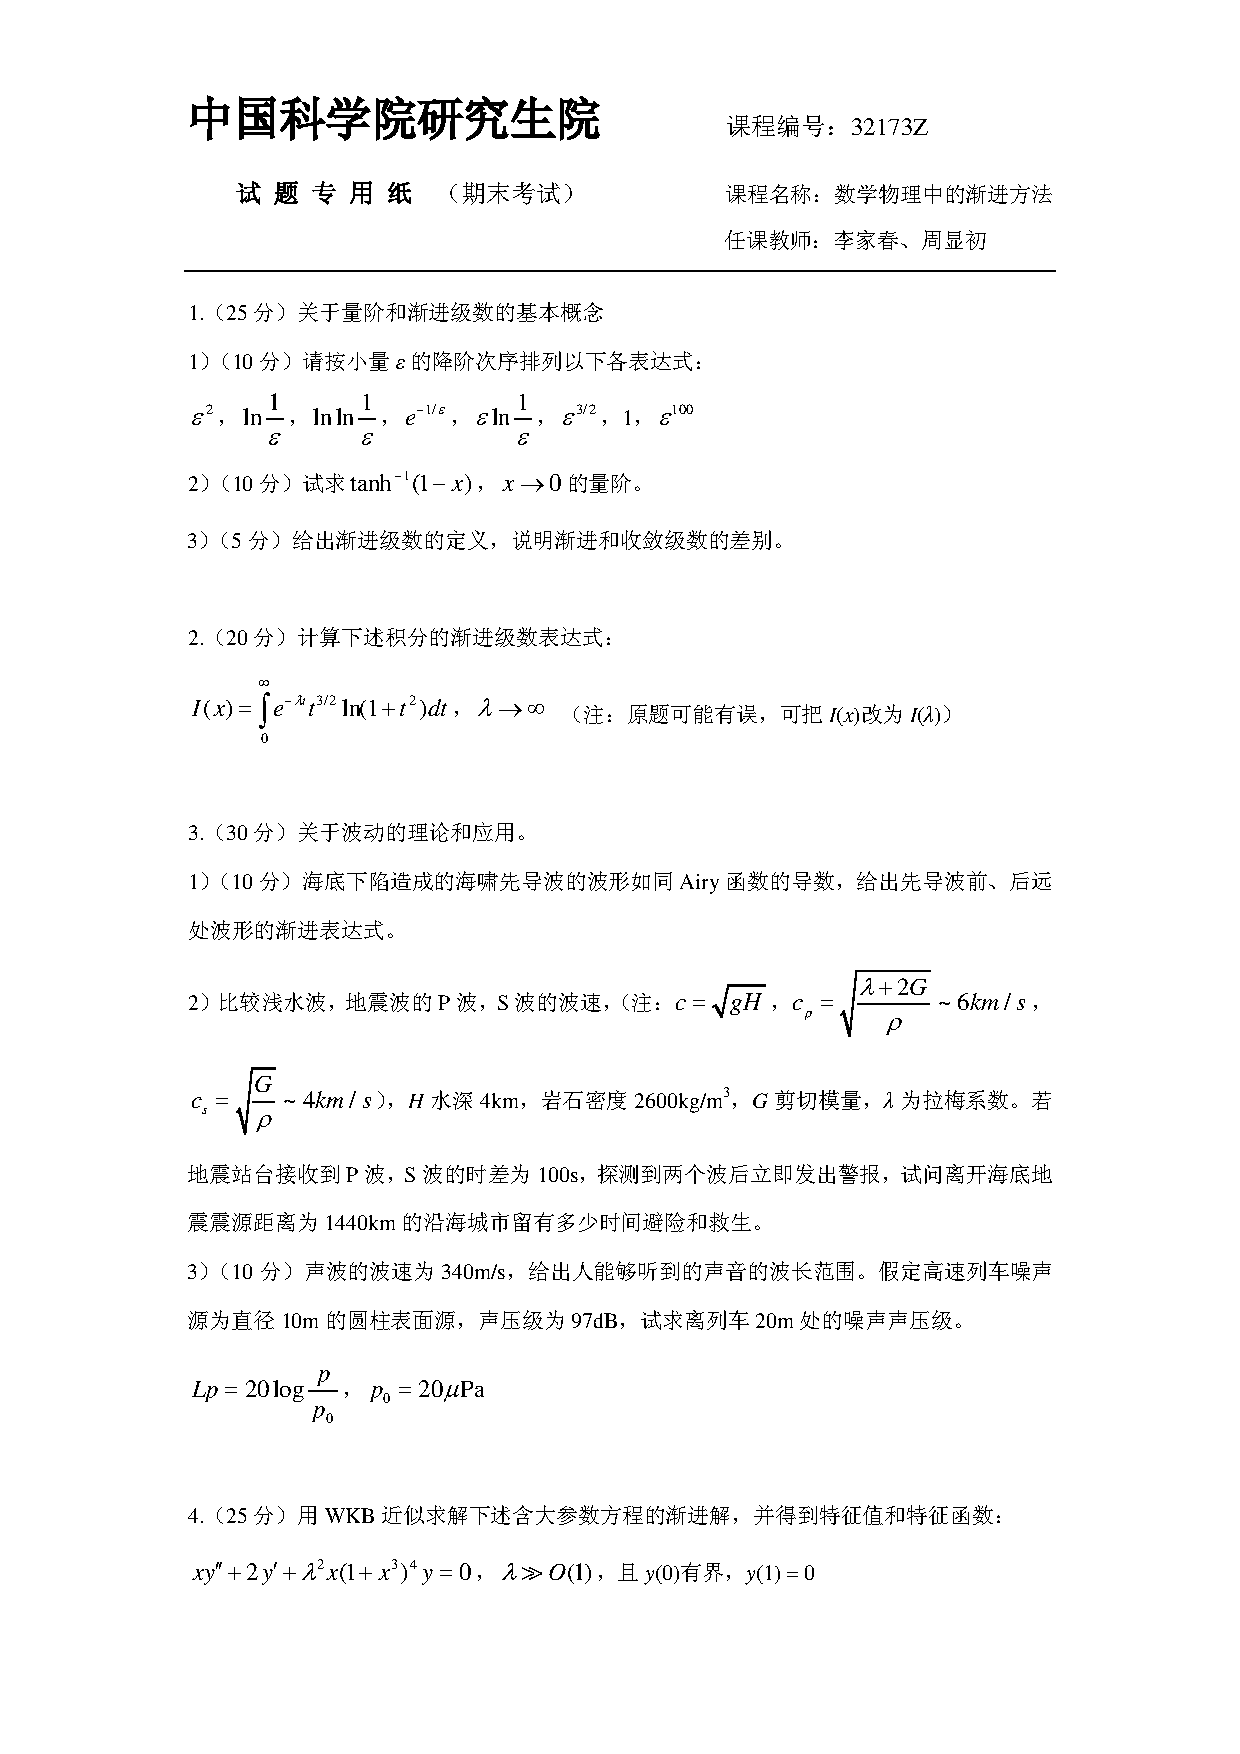
\includegraphics[width=0.95\textwidth]{exam2.pdf}}
\end{center}
